\subsection{Arquitectura  del servidor}

El servidor se ha implementado con Spring Boot \cite{spring}, un framework que permite la creación de aplicaciones en Java de una forma más sencilla. Esta simplifica el proceso de gestión de las dependencias, permitiendo que nos centremos lo máximo posible en el desarrollo de la aplicación.

\begin{figure}[H]
\centerline{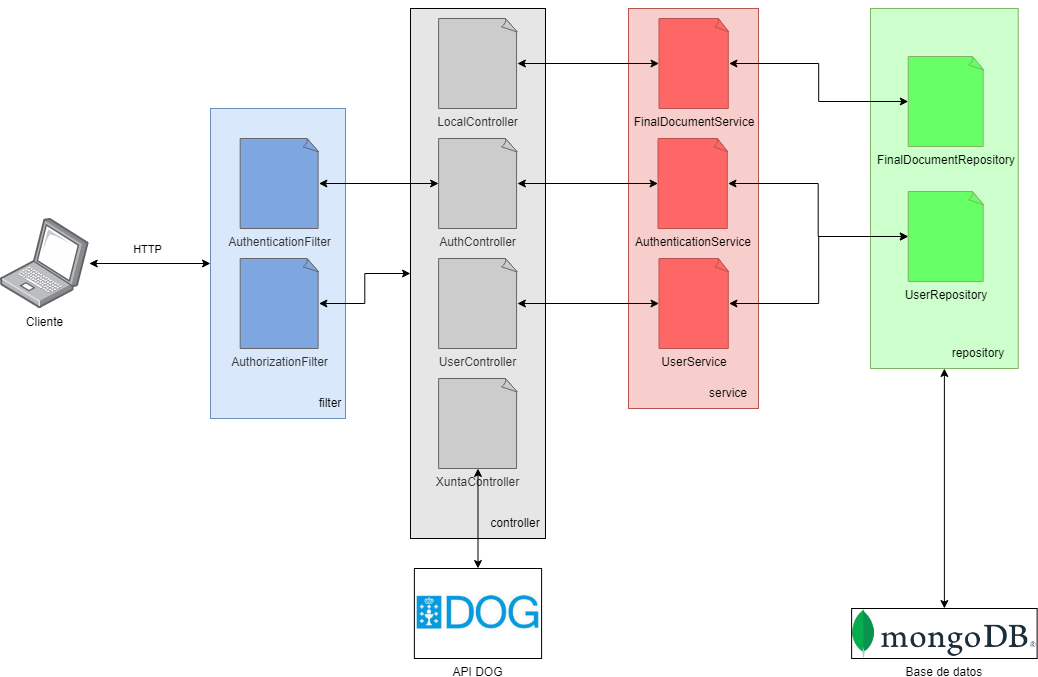
\includegraphics[width=15cm]{figuras/diseño/FicherosServidor.png}}
\caption{Arquitectura del servidor.}
\label{enlaceArquitecturaServidor}
\end{figure}

El servidor está dividido en un conjunto de directorios, cada uno con una función diferente. 
\\

Todas las dependencias del servidor son definidas en el archivo {\bf build.gradle}. Dichas dependencias son tratadas por Gradle \cite{gradle}, un gestor de dependencias en aplicaciones de Java.
\\

En el subdirectorio {\bf main}, encontraremos una carpeta denominada {\bf resources}. En el fichero contenido en ella, se define el nombre de la base de datos que ha de utilizar la aplicación.
\\

Si accedemos al directorio {\bf java/tfg/project}, encontramos el contenido principal del servidor. El archivo {\bf Application} es el encargado de desplegar el servidor, pues contiene la función main del programa.
\\

En el directorio {\bf Config}, se localizan archivos de configuración del propio servidor, tales como aspectos de seguridad, documentación, privacidad, etc. 
\\

Otro directorio es el {\bf Filter}, donde se tratan distintos aspectos de seguridad con respecto a los usuarios que utilizan la aplicación, como puede ser el inicio de sesión, gestión de contraseñas o comprobación de roles.
\\

En la carpeta {\bf Model} encontramos los distintos objetos que conforman la base de la aplicación. Podemos destacar entre ellos el objeto {\bf FinalDocument}, que está formado por todos los atributos de la ley, y {\bf User}, que es el objeto utilizado para gestionar los usuarios. Todos estos objetos son empleados por las clases definidas en las carpetas {\bf Controller, Service y Repository}.
\\

En la carpeta {\bf Controller}, encontramos todos los archivos encargados de redirigir las llamadas a los servicios necesarios en la carpeta Service. Estos se encargan de localizar cualquier llamada al servidor (GET, POST, ...), y entregarla a los servicios.
\\

Con respecto al directorio {\bf Service}, este contiene los archivos donde se localizan los servicios web. Aquí se implementa la lógica de negocio de la aplicación, y no se conserva estado. Es llamada por los controladores, y solicita información a los repositorios donde se almacena toda la información.
\\

Como último directorio, se encuentra {\bf Repository}, donde se almacenan los ficheros que se encargan del acceso y almacenamiento de datos. Estos gestionan la conexión con la base de datos para poder obtener/almacenar información en ella.
\\

En resumen, las funcionalidades de los controladores, servicios y repositorios son las siguientes:
\begin{itemize}
    \item {\bf LocalController, FinalDocumentService y FinalDocumentRepository}: se encargan de gestionar las operaciones relacionadas con las leyes.
    \item {\bf UserController, UserService y UserRepository}: se encargan de gestionar las operaciones relacionadas con los usuarios.
    \item {\bf AuthController, AuthenticationService y UserRepository}: se encargan de gestionar las operaciones relacionadas con aspectos de seguridad respecto a los usuarios, como el inicio de sesión.
    \item {\bf XuntaController}: se encarga de gestionar las llamadas a la API de la Xunta.
\end{itemize}

\subsubsection{Documentación de la API del servidor}

La documentación de la API del servidor se ha realizado con Swagger \cite{swagger}, siendo posible consultarse en mayor detalle accediendo a la URI ``/swagger-ui/index.html''. Por ejemplo, en el caso de desplegar el servidor localmente, el enlace sería {\it \url{http://localhost:8080/swagger-ui/index.html}}. No obstante, se realiza aquí un pequeño resumen de las principales operaciones ofrecidas.

\begin{figure}[H]
\centerline{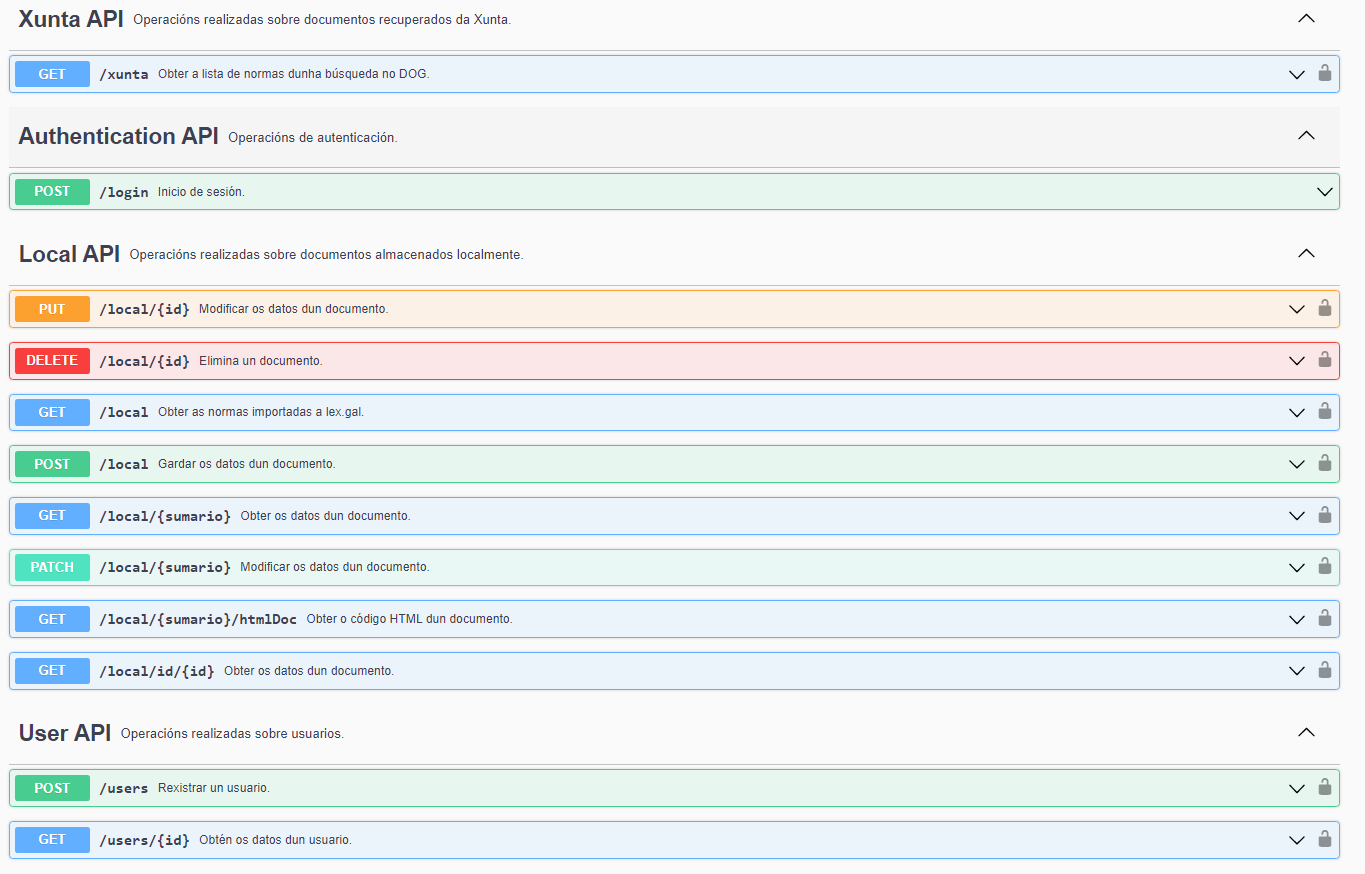
\includegraphics[width=15cm]{figuras/diseño/APIServidor.PNG}}
\caption{API del servidor.}
\label{enlaceAPIServidor}
\end{figure}

\begin{itemize}
    \item Para las operaciones del DOG se realiza un GET para obtener las normas buscadas. Es necesario estar autenticado. La URI de acceso es {\it /xunta}.
    \item Para los aspectos de autenticación no es necesario estar autenticado. La única operación existente es un POST para realizar el login. Se obtiene un token JWT \cite{jwt} para mayor seguridad (NFR-10). La URI de acceso es {\it /login}.
    \item Las operaciones relacionadas con leyes son: GET para obtener todos los datos, solo el sumario, el documento HTML de la ley y el id de la ley. POST se utiliza a la hora de almacenar nuevas leyes. PUT para modificar una ley completa. PATCH para modificar parcialmente atributos de una ley. DELETE para eliminar documentos. La URI de acceso general es {\it /local}.
    \item En cuanto a los usuarios, solo se permite realizar GET para obtener los datos de un usuario, y POST para crear nuevos usuarios. La URI de acceso general es {\it /users}.
\end{itemize}